\documentclass{standalone}


\usepackage{tikz}
\usetikzlibrary{shapes.geometric, arrows}
\usetikzlibrary{positioning}


\tikzstyle{startstop} = [rectangle, rounded corners, minimum width=2cm, minimum
height=0.5cm,text centered, draw=black]

\tikzstyle{io} = [trapezium, trapezium left angle=70, trapezium right angle=110, minimum
width=2.5cm, minimum height=0.5cm, text centered, text width = 1.5cm, draw=black]

\tikzstyle{process} = [rectangle, minimum width=2cm, minimum height=0.5cm, text centered,
text width = 1cm, draw=black]
\tikzstyle{decision} = [diamond, minimum width=2cm, minimum height=0.5cm, text centered,
draw=black]

\tikzstyle{block1} = [rectangle, rounded corners, minimum width=0.5cm, minimum
height=0.25cm,text centered, draw=black]

\tikzstyle{block2} = [rectangle, rounded corners, minimum width=2.5cm, minimum
height=3.6cm,text centered, draw=black]



\tikzstyle{arrow} = [thick,->,>=stealth]


\begin{document}

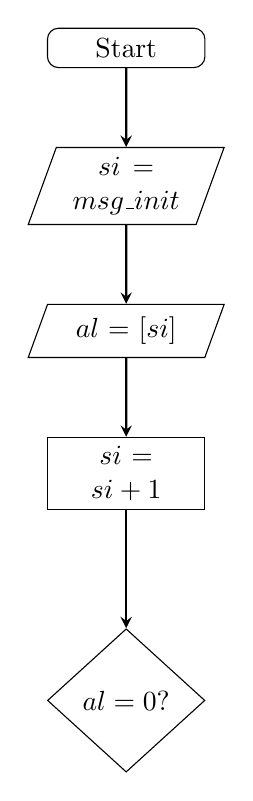
\begin{tikzpicture}
    \node (start) [startstop]  {Start};
    \node (in1) [io, below=of start,align=center] {$si=msg\_init$};
    \node (in2) [io, below=of in1, align=center] {$al=[si]$};
    \node (pro1) [process, below=of in2] {$si=si+1$};
    \node (dec1) [decision, below=of pro1, yshift = -0.5cm] {$al=0?$};
    
    \draw[arrow] (start) -- (in1);
    \draw[arrow] (in1) -- (in2);
    \draw[arrow] (in2) -- (pro1);
    \draw[arrow] (pro1) -- (dec1);
    
\end{tikzpicture}
\end{document}

%%% Local Variables:
%%% mode: latex
%%% TeX-master: t
%%% End:
